% Created 2023-02-27 Mon 18:52
% Intended LaTeX compiler: pdflatex
\documentclass[11pt]{article}
\usepackage[utf8]{inputenc}
\usepackage[T1]{fontenc}
\usepackage{graphicx}
\usepackage{longtable}
\usepackage{wrapfig}
\usepackage{rotating}
\usepackage[normalem]{ulem}
\usepackage{amsmath}
\usepackage{amssymb}
\usepackage{capt-of}
\usepackage{hyperref}
\author{Yusheng Zhao}
\date{\today}
\title{Homework 1}
\hypersetup{
 pdfauthor={Yusheng Zhao},
 pdftitle={Homework 1},
 pdfkeywords={},
 pdfsubject={},
 pdfcreator={Emacs 28.2 (Org mode 9.6)}, 
 pdflang={English}}
\begin{document}

\maketitle
\tableofcontents


\section{Problem 1}
\label{sec:org093bcec}
\begin{itemize}
\item Name: SPERM WHALE MYOGLOBIN F46V N-BUTYL ISOCYANIDE AT PH 9.0
\item ID: 101M
\begin{figure}[htbp]
\centering
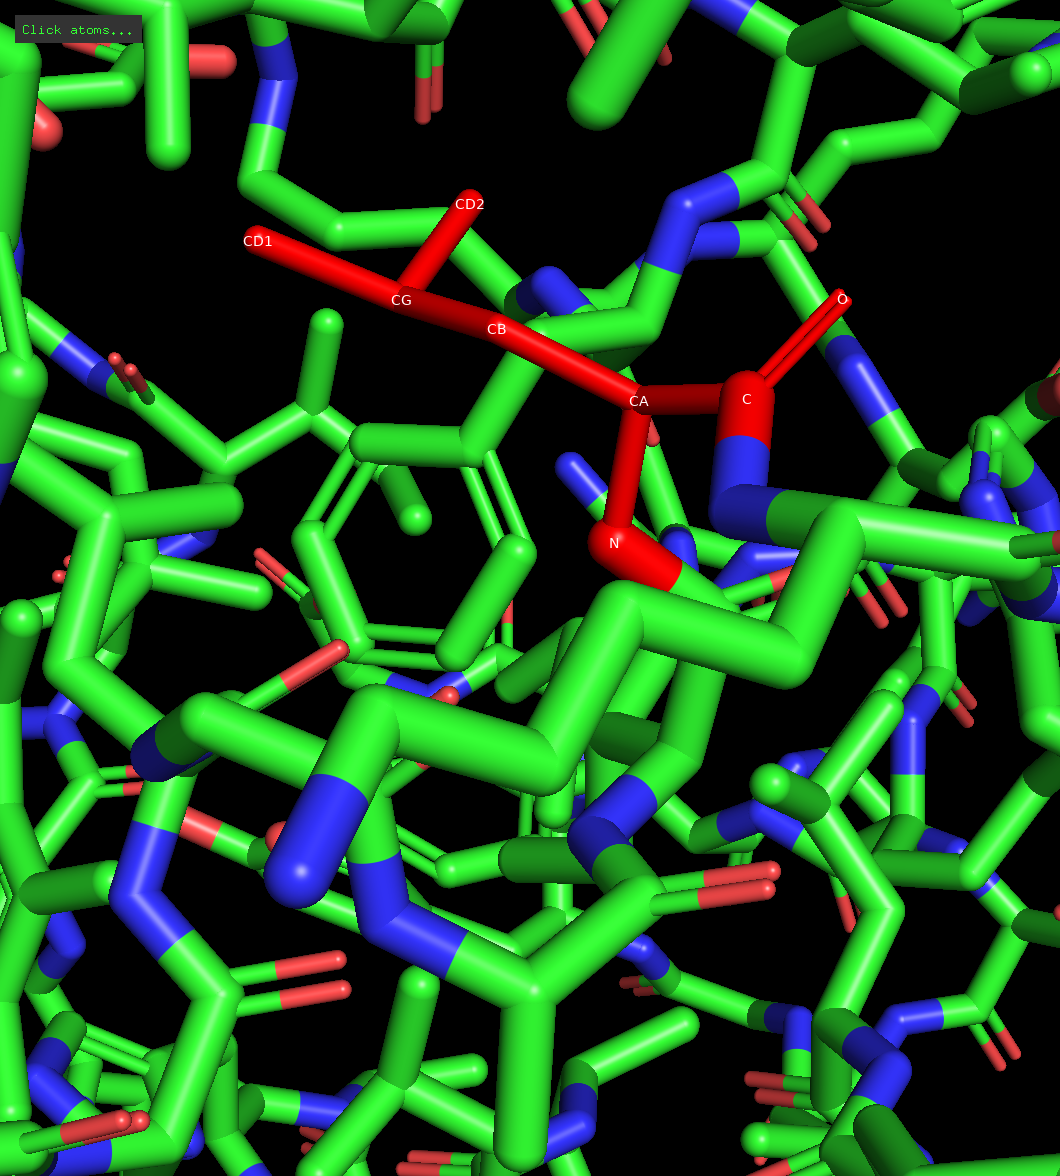
\includegraphics[width=.9\linewidth]{./sticks.png}
\caption{Illustration of molecule with sticks, atoms names of one amino acid labeled.}
\end{figure}

\begin{figure}[htbp]
\centering
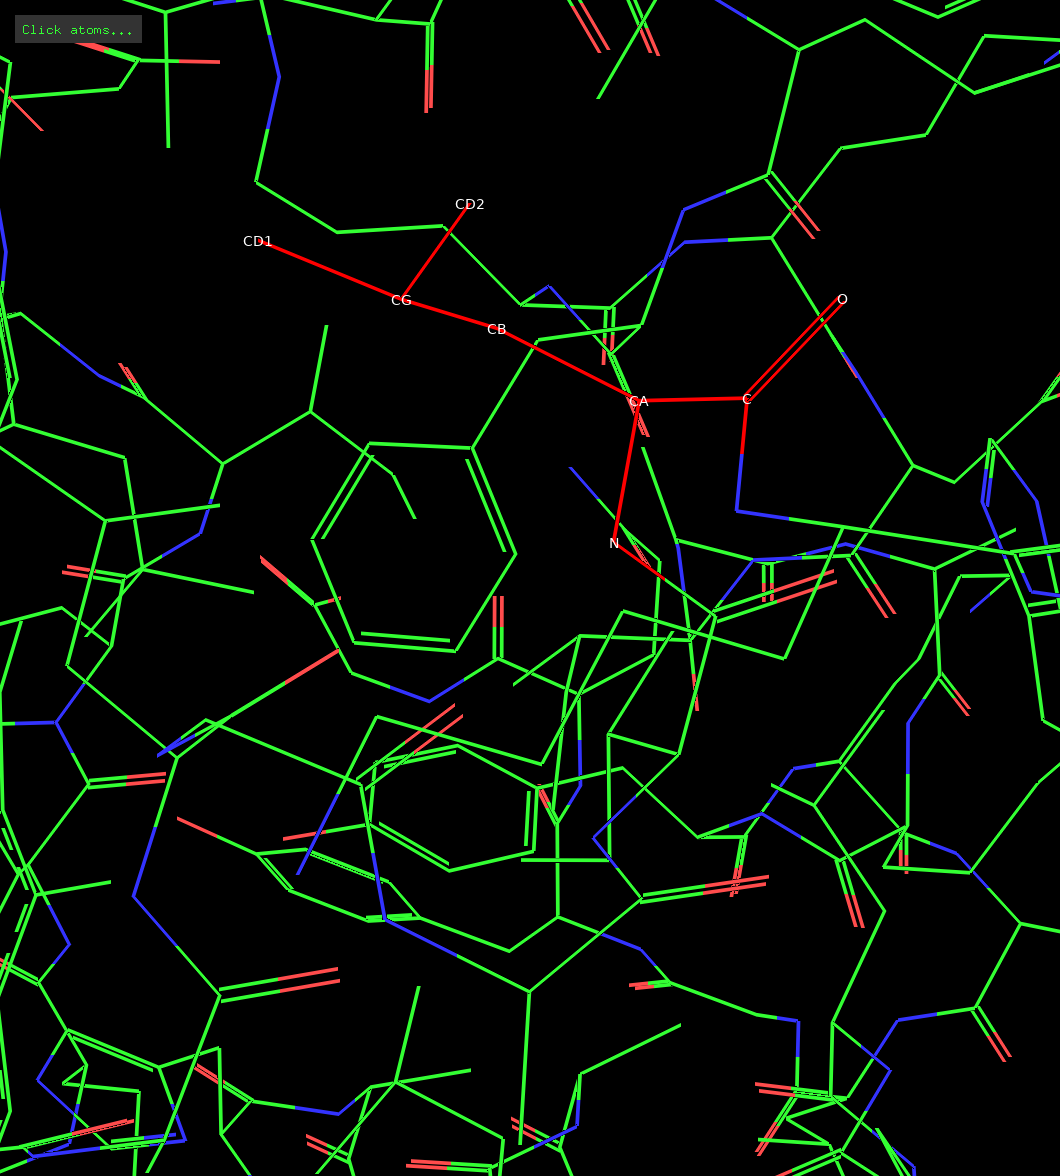
\includegraphics[width=.9\linewidth]{./lines.png}
\caption{Illustration of molecule with lines, atoms of one amino acid labelled}
\end{figure}

\begin{figure}[htbp]
\centering
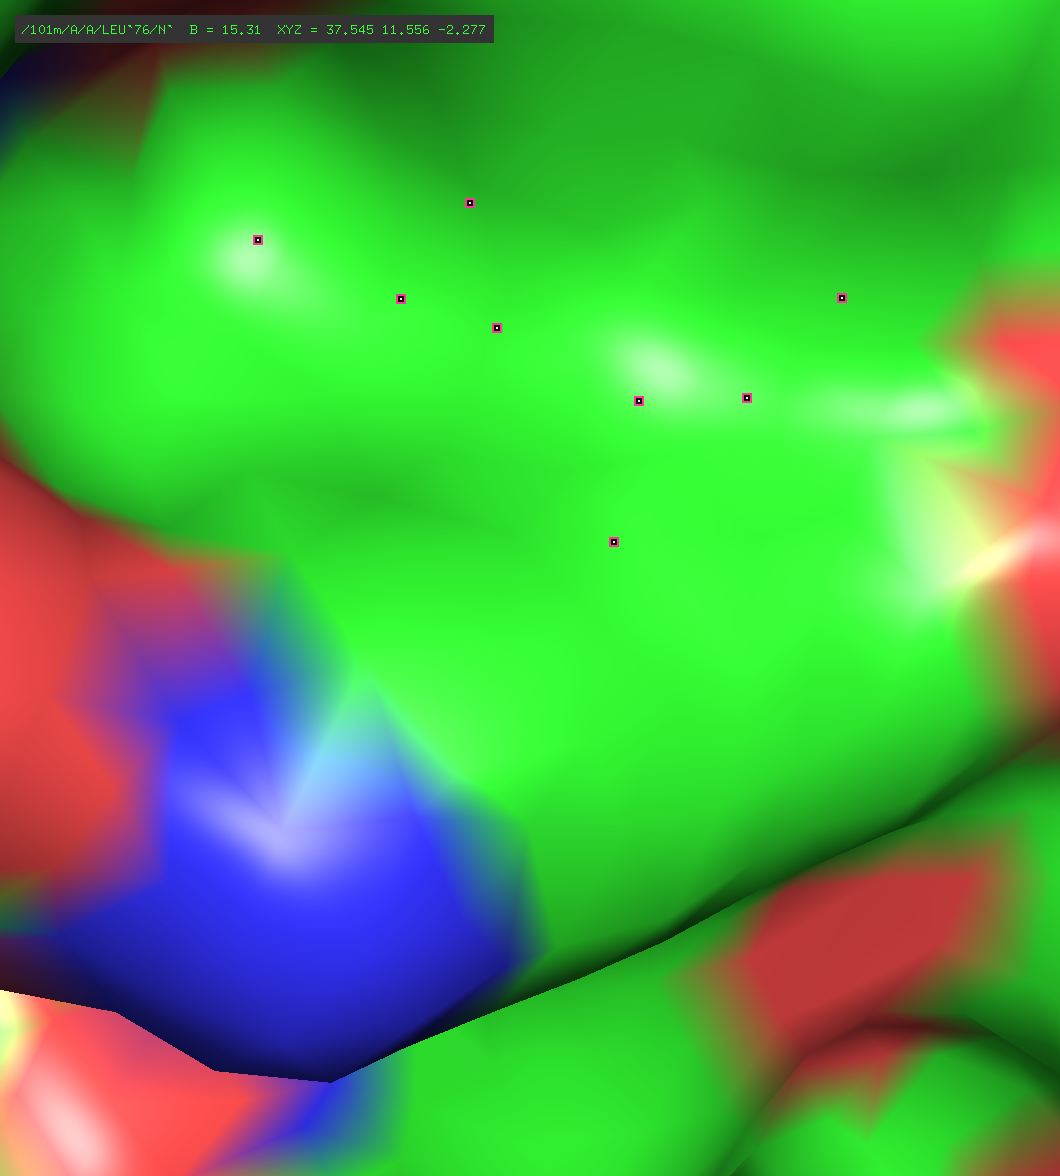
\includegraphics[width=.9\linewidth]{./surfaces.png}
\caption{Illustration of molecule with surfaces, atoms and names hidden under surface}
\end{figure}
\end{itemize}

\begin{figure}[htbp]
\centering
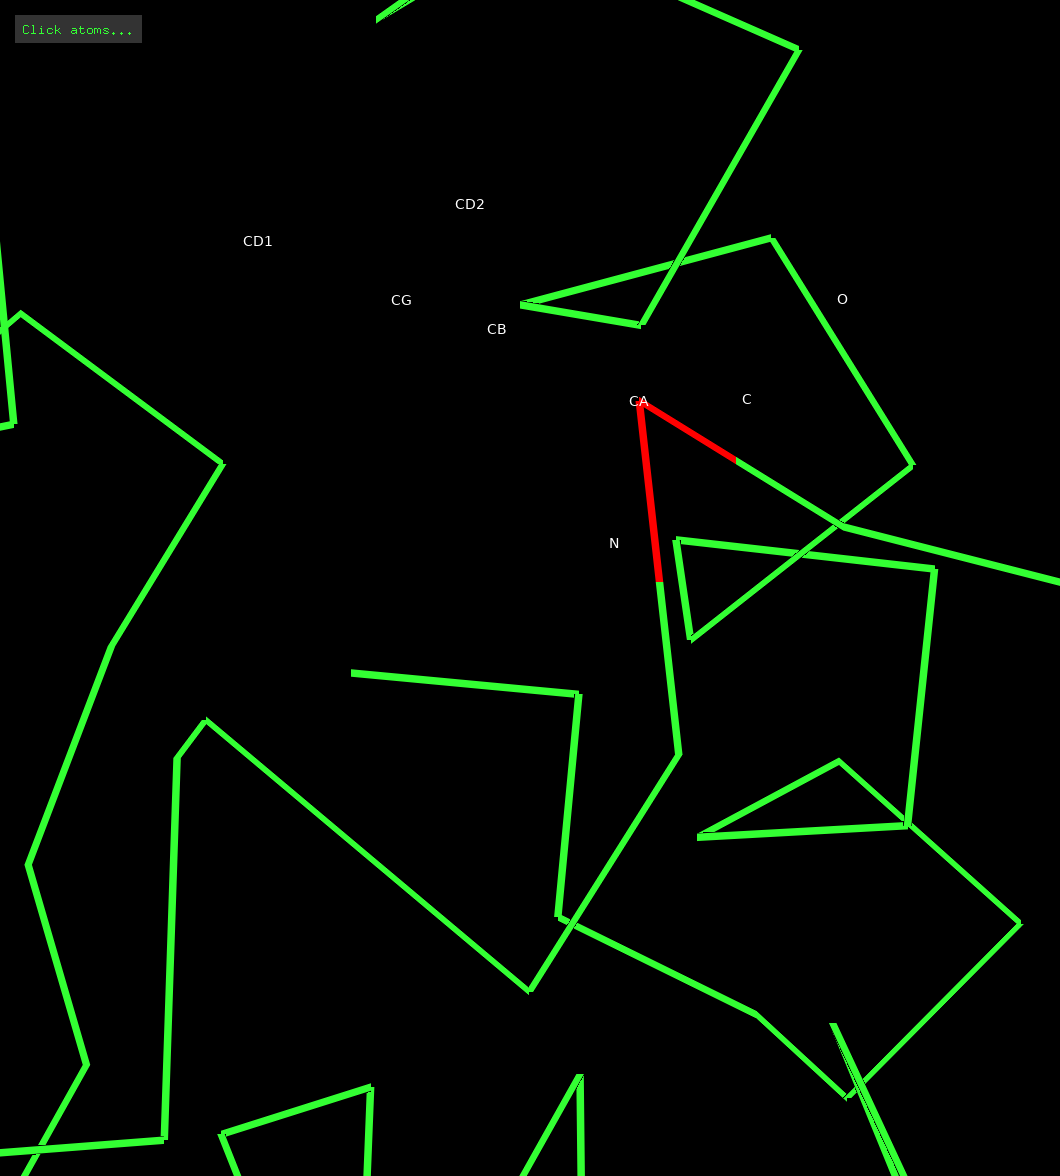
\includegraphics[width=.9\linewidth]{./ribbons.png}
\caption{Illustration of molecule with ribbons, atoms hidden but labels are in view.}
\end{figure}

\section{Problem 2}
\label{sec:orgf175cd7}
Since \(\beta \equiv 1/(k_{B}T)\), \(\partial \beta = -
\frac{1}{k_{B}T^{2}}\partial T\).
\begin{align}
c_{v}    & \equiv \frac{\partial <U>}{\partial T} \\
        & =  - \frac{1}{k_{B}T^{2}} \frac{\partial <U>}{\partial \beta} \\
        & =  \frac{1}{k_{B}T^{2}} \frac{\partial }{\partial \beta} (\frac{\partial ln(Z)}{\partial \beta}) \\
        & =  \frac{1}{k_{B}T^{2}} \frac{\partial }{\partial \beta} (\frac{\partial Z /\partial \beta}{Z}) \\
 & = \frac{1}{k_{B}T^{2}} \frac{\frac{\partial^{2}Z}{\partial\beta^{2}} Z - (\frac{\partial Z}{\partial\beta})^{2}}{Z^{2}} \\
 & = \frac{1}{k_{B}T^{2}} (\frac{\frac{\partial^{2}Z}{\partial\beta^{2}}}{Z} - (\frac{\partial Z}{\partial \beta} / Z)^{2}) \\
& = \frac{1}{k_{B}T^{2}} (<U^{2}> - <U>^{2})
\end{align}

For the last step, we used the fact that \(Z = \sum e^{-U\beta}\), taking
derivative with respect to \(\beta\) twice will bring down \(U^{2}\).
\end{document}